
\documentclass[12pt]{report}

%  PACKAGES ==========================================================
\usepackage{amsmath,amsthm,amsfonts,amssymb,amscd,mathrsfs,mathtools}  % Math packages
\usepackage{natbib}         % for references
\usepackage{multirow}       % for equaitons
\usepackage{wrapfig}        % to wrap figure with text
\usepackage{graphicx}       % allows adding graphics to the text
\usepackage{verbatim}       % Allows quoting source with commands.
\usepackage{makeidx}        % Package to make an index.
%\usepackage{psfig}          % Allows inclusion of eps files.
%\usepackage{epsfig}         % Allows inclusion of eps files.
%\usepackage{epstopdf}       % allows .eps figures in the text
%\usepackage{pdftex}        % allows .eps figures in the text
%\usepackage{pdflatex}      % allows .eps figures in the text

\usepackage{url}            % Allows good typesetting of web URLs.
\usepackage{subfigure}      % to have multi figures in the same figure
\usepackage{comment}        % allow commnets in the file
%\usepackage[linesnumbered,lined,boxed,commentsnumbered]{algorithm2e} % To include algorithm - this one is more professional, but we cannot break the algorithm in pages
\usepackage{float}
%\usepackage{algorithm}      % To include algorithm 
%\usepackage{algpseudocode}  % for algorithms 
\usepackage[bookmarks]{hyperref}  % to add bookmarks to all references
\usepackage{ragged2e}       % Text justifying
\usepackage{color}
\usepackage{ctable}
%\usepackage{pmat}
%\usepackage{ulem}
%\usepackage[retainorgcmds]{IEEEtrantools}
%\usepackage[dvips]{geometry}
%\usepackage{lscape}
%\setcounter{MaxMatrixCols}{40}

%\usepackage[framed,numbered,autolinebreaks,useliterate]{mcode} % Add a Matlab code
%\usepackage{eucal} 		    % Euler fonts
%\usepackage{setspace}
%\usepackage{algorithm,algorithmicx,algpseudocode}   % algorithms
%\usepackage{draftcopy}		% Uncomment this line to have the
                          %   word, "DRAFT," as a background
                          %   "watermark" on all of the pages of
                          %   of your draft versions. When ready
                          %   to generate your final copy, re-comment
                          %   it out with a percent sign to remove
                          %   the word draft before you re-run
                          %   Makediss for the last time.

% Extra stuff =======================================================
%\allowdisplaybreaks  % to break long equations into two pages


% = Constants ========================================================
\renewcommand\textfraction{.1}
\setcounter{totalnumber}{5}
\renewcommand{\floatpagefraction}{.8}

%\setlength{\bibsep}{0pt plus 0.3ex}    % This line reduces the spacing between the references  - Remove in the final version

% = Figure spacing ==================================================
\renewcommand{\subfigbottomskip}{-2pt}
\renewcommand{\subfigcapskip}{-2pt}
\renewcommand{\subfigcapmargin}{0pt}

%\setlength{\belowcaptionskip}{-10pt}

\setlength{\textfloatsep}{14pt plus 1.0pt minus 2.0pt}
\setlength{\intextsep}{14pt plus 1.0pt minus 2.0pt}
\setlength{\floatsep}{14pt plus 1.0pt minus 2.0pt}


% General information ===============================================
\author{Babak Poursartip}
%\address{babakp@utexas.edu}

\title{My ML studies}

\makeatletter		% Starts section where @ is considered a letter
          			% and thus may be used in commands.
\def\square{\RIfM@\bgroup\else$\bgroup\aftergroup$\fi
  \vcenter{\hrule\hbox{\vrule\@height.6em\kern.6em\vrule}%
                                              \hrule}\egroup}
\makeatother		% Ends sections where @ is considered a letter.
			          % Now @ cannot be used in commands.

%\makeindex      % Make the index


% Beginning =========================================================
\begin{document}

\justifying


%\titlepage    % Produces the title page.
\maketitle



% Tables ============================================================
\pdfbookmark{\contentsname}{toc}  % To bookmark the table of contents
\tableofcontents                  % Table of Contents will be automatically
%\listoftables                     % List of Tables and List of Figures will be placed
%\listoffigures                    % here, if applicable.
%\listofalgorithms                 % List of algorithms
%\addcontentsline{toc}{chapter}{List of Algorithms}  % This command includes the list of algorithms in the table of content

% Chapters ==========================================================
%\include{chapter1_Introduction}
\chapter[Introduction]{Introduction}
\label{ch:ML}
\noindent

\section{General}

\begin{itemize}
	\item Supervised learning: functional approximation from labeled data. 
	\item Unsupervised learning: functional description.
	\item Reinforcement learning: Learning from delayed reward. 
\end{itemize}


\section{Supervised learning}
\label{sec:sl}
There are two types of supervised learning:

\begin{itemize}
\item classification: taking some inputs and mapping it to some discrete label. (true of false, male or female, etc.)
\item regression: continuous valued function. Mapping from input to some \textbf{real number}. Something like age is more like discrete number, so, it is also classification. 
\end{itemize}

\subsection{Terms}
\begin{itemize}
\item Instances: Inputs-pictures, pixels, etc.
\item Concept: A set of functions that maps inputs to outputs.
\item Target concept: The actual function that can map inputs to outputs. This is the actual answer.
\item Hypothesis class: Set of all the functions that we are going to think about. 
\item Sample (Training set): A set of instances with correct labels.
\item Candidate: The best approximation of the target concept.
\item Testing set: A set of instances with correct labels that was not visible to the learning algorithm during the training phase. It’s used to determine the algorithm performance on novel data. we can argue that we learned something by memorization, but indeed, we just memorized the concepts. What we want is generalization. 
\end{itemize}


\chapter[Decision tree]{Decision tree}

\section{Intro}
\label{sec:dt}

First, we need to come up with a set of features for our decision tree. 


\textbf{Representation vs Algorithm:}

A decision tree is a structure of nodes, edges and leaves that can be used to represent the data.
\begin{itemize}
\item Nodes represent attributes where you ask a question about it. (vehicle length, vehicle height, number of doors, etc.).
\item Edges represent values. (A specific value for each attribute)
\item Leaves represent the output/answer (vehicle’s type).
\end{itemize}

A decision tree algorithm is a sequence of steps that will lead you to the desired output. To form a decision tree, we need to come up with the attributes that can split the space, roughly in half. 
\begin{itemize}
\item Pick the best attribute (the one that can split the data roughly in half). If this attribute added no valuable information (not a good split), it might cause overfitting.
\item Ask a question about this attribute.
\item Follow the correct answer path.
\item Loop back to (1) till you narrow down the possibilities to one answer (the output).
\end{itemize}
Note that the usefulness of a question depends upon the answers we got to previous questions.
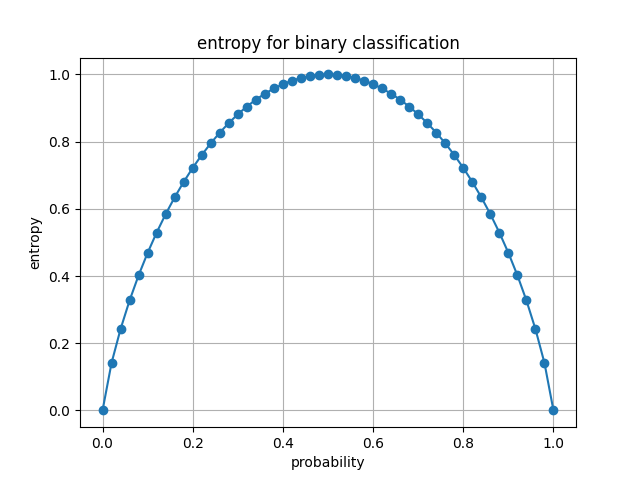
\includegraphics[scale=0.5]{entroy.png}


\section{Expressiveness}

\begin{itemize}
	\item Decision trees can basically express any function using the input attributes.
	\item For Boolean functions (AND, OR, XOR, etc.), the truth table row will be translated into a path to a leaf.
	\item How many decision trees we can generate for a specific function/problem? Decision tree hypothesis space is very huge $(2^{(2^{n})})$, this why we need to design algorithms to efficiently search the hypothesis space for the best decision tree. 
\end{itemize}

\section{ID3 algorithm to create a decision tree}
ID3 builds decision trees using a top-down, greedy approach. The greedy part of the approach comes from the fact that it will decide which attribute should be at the root of the tree by looking just one move ahead. It compares all available attributes to find which one classifies the data the best, but it doesn’t look ahead (or behind) at other attributes to see which combinations of them classify the data the best.

Pseudocode:
\begin{enumerate}
\item Pick the best attribute A (The definitions of best attribute comes later). To select this attribute, a statistical test is used to determine for each attribute how well it alone classifies the training examples.
\item Split the data into subsets that correspond to the possible values of the best attribute.
\item Assign A as a decision attribute for a node.
\item For each value of A, create a descendant node.
\item Sort training examples to leaves.
\item If examples perfectly classified --	Stop -- else --Iterate over leaves	
\end{enumerate}	


How to find the best attribute for the decision tree at each level: \\
There are a couple of option. The most common method is called information gain: a measure that expresses how well an attribute splits the data into groups based on classification (for ex., if an attribution returns low info. gain, if it divides samples to two classes with a even yes/no, but the info gain is high, if each class has more of yeses or nos).

It quantifies the reduction in randomness (Entropy) over the labels we have with a set of data, based upon knowing the value of a particular attribute. A mathematical way to measure the gain, is entropy. It measures the homogeneity of a data set S's  classifications. It ranges from 0, which means that all of the classifications in the data set are the same (either yes or no), to $log_{2}$ of the number of different classifications, which means that the classifications are equally distributed within the data set. For a binary classification the entropy is only $log_{2} 1 = 1$ (if yes and no samples are equally divided). entropy is calculated as follows: 

\begin{equation}
Entropy(S) = \sum_{i=1}^{c} -p_{i} \; log_{2} (p_{i})
\end{equation}
where:
\begin{itemize}
\item c corresponds to the number of different classifications 
\item $p_{i}$ corresponds to the proportion of the data with the classification i
\end{itemize}

Here is the plot of entropy for a binary classifier, as the proportional of yes and no samples change:

Information gain measures the reduction in entropy that results from partitioning the data on an attribute A, which is another way of saying that it represents how effective an attribute is at classifying the data. Given a set of training data S and an attribute A, the formula for information gain is:

\begin{equation}
	Gain(S,A)  = Entropy(S) - \sum_v  \frac{|S_v|}{|S|} \; Entropy(S_v)
\end{equation}

where $v$ is all the possible values of attribute A (for example, sunny, cloudy, rainy), and $S_v$ is the total number of samples (regardless of the value of the sample) corresponding to this value of attribute (for example sunny). We want to maximize information gain, so we want the entropies of the partitioned data to be as low as possible, which explains why attributes that exhibit high information gain split training data into relatively heterogeneous groups.

As the size of the training data and the number of attributes increase, it becomes likelier that running ID3 on it will return a suboptimal decision tree.

\section{Extending ID3 algorithm}
Small tweaks allow ID3 to handle continuous attributes, missing attribute values, data that doesn’t work particularly well with
information gain, and more.

For continuous attributes, we can classify the attributes based on thresholds. 

If the data for some attributes is missing, we can choose the most popular data for the missing item. Two options here: does not take the classification into account, or choose the most popular value for the same classification. 
Another method to deal with the missing data, is assigning the probability of each value of the attribute to the missing entries. 


\section{over-fitting}
There are two popular approaches to avoid this in decision trees: stop growing the tree before it becomes too large or prune the tree after it becomes too large. Typically, a limit to a decision tree’s growth will be specified in terms of the maximum number of layers, or depth, it’s allowed to have.

The data available to train the decision tree will be split into a training set and test set and trees with various maximum depths will be created based on the training set and tested against the test set.

Pruning the tree, on the other hand, involves testing the original tree against pruned versions of it. Leaf nodes are taken away from the tree as long as the pruned tree performs better against test data than the larger tree.


Changing the information gain formula:
The information gain formula used by the ID3 algorithm treats all of the variables the same, regardless of their distribution and their importance. This is a problem when it comes to continuous variables or discrete variables with many possible values because training examples may be few and far between for each possible value, which leads to low entropy and high information gain by virtue of splitting the data into small subsets, but results in a decision tree that might not generalize well.

One successful approach to deal with this is using a formula called GainRatio in the place of information gain. GainRatio tries to correct for information gain’s natural bias toward attributes with many possible values by adding a denominator to information gain called SplitInformation. SplitInformation attempts to measure how broadly partitioned an attribute is and how evenly distributed those partitions are. In general, the SplitInformation of an attribute with n equally­distributed values is log 2 n . These relatively large denominators significantly affect an attribute’s chances of being the best attribute after an iteration of the ID3 algorithm and help to avoid choices that perform particularly well on the training data but not so well outside of it.

\begin{gather*}
	GainRatio(S,A)  = \frac{Gain(S,A)}{SplitInformation(S,A)} \\
	SplitInformation(S,A) = - \sum_{i=1}^c \frac{|S_i|}{S} \; log_2\frac{|S_i|}{|S|}
\end{gather*}


\section{BIAS (Inductive bias)}
Two types of bias: restriction bias (hypophysis), and preference bias (prefer a subset of hypophisys, this is inductive).

Bias of ID3 are: 
\begin{itemize}
\item it prefers the decision tree with good splits at top (even if a bad split generates the same outcome).
\item it prefers correct outcome over incorrect. 
\item it prefers shorter trees (comes from that fact that we use good splits from the top).
\end{itemize}



% Appendix ==========================================================
%\appendices
%\include{appendix_Matrices}


%\renewcommand*{\bibfont}{\footnotesize}  % This command reduces the font size. Comment this for the final draft
%\renewcommand*{\bibfont}{\scriptsize}  % This command reduces the font size. Comment this for the final draft
\addcontentsline{toc}{chapter}{Bibliography}
\bibliographystyle{plain}  				% Here the bibliography  %
\bibliography{reference}        	% is inserted.			     %
\index{bibliography}

\end{document}

